\documentclass[11pt]{article}
\usepackage[brazilian]{babel}
\usepackage[utf8]{inputenc} %Deixa eu colocar letras com ascentos
\usepackage[T1]{fontenc}
\usepackage{amsmath}
\usepackage{color}
\usepackage{graphicx}


\title{Relatório - EP Fase 2 \\ Laboratório de Programação 2}



\begin{document}

\maketitle

\section{Integrantes}

\begin{itemize}

\item Victor Sanches Portella - Nº USP: 7991152

\item Lucas Dário - Nº USP: 7990940

\item Ruan Costa - Nº USP: 7990929

\end{itemize}

\section{Introdução}

Neste relatório temos como objetivo dar uma explicação concisa sobre a organização das classes no funcionamento do programa atualmente. Para isso, explicaremos o funcionamento do programa inteiro, e iremos nos aprofundar nos assuntos que forem necessários.


\section{Funcionamento}

Nessa fase o EP ainda não têm o funcionamento de um jogo em si, mas já é possível ver diversos robôs agindo em paralelo. Para isso, o script em Perl\footnote{Explicação do mesmo feita mais a frente} traduz diversos programas para um arquivo chamado \textbf{\color{red}Main.java}. 

Todos os robôs traduzidos serão colocados no mesmo time. Ao rodar o programa, os programas de cada robô serão executados até o fim. Quando todos os robos tiverem encerrado sua execução, o programa será finalizado.

Cada robô imprime as instruções que executou para que assim possamos acompanhá-las.

\section{Classes}

\subsection{Classe Arena}


Essa classe representa a Arena em si. Nela, temos os seguintes atributos:

\begin{itemize}

	\item \textbf{Mapa}: Objeto do tipo \textbf{\color{red}Mapa} que representa o mapa em si. Nesse objeto existe uma matriz de Terrenos, cada um contendo informações como robôs naquele terreno, assim como cristais, bases, etc. Melhores explicações sobre esse objeto serão dadas mais a frente.
	
	\item \textbf{List<{\color{red}Robos}>}: Objeto do tipo \textbf{\color{red}List} usado como uma lista de objetos do tipo \textbf{\color{red}Robo}. Essa lista contêm todos os robôs em jogo.
	
	\item \textbf{Tempo}: Uma variável inteira representando o número de rodadas já passadas. O valor inicial dessa variável é 0 e, a cada rodada, é incrementada em 1.

\end{itemize}

Principais métodos dessa classe:

\begin{itemize}

\item \textbf{Arena({\color{red}Mapa})}: Construtor da classe. Recebe uma mapa, e retorna uma arena vazia, ou seja, com nenhum robo, o tempo é iniciado com 0, e o mapa passado é definido como o mapa da arena.

\item \textbf{{\color{red}void} atualiza()}: Função que faz a Arena executar uma rodada. Atualmente, essa função percorre a lista de robôs de forma aleatória, executando em cada robô uma instrução de máquina. Em caso de conflito de instruções, tem preferência o robô que for executado primeiro naquela iteração.

\item \textbf{{\color{red}void} sistema({\color{red}Operacao})}: Função chamada pelos robôs para fazerem chamadas ao sistema. Toda vez que os robôs tentam executar uma ação que influencia seu exterior, ele só pode fazê-la chamando esse método. O objeto do tipo \textbf{\color{red}Operacao} recebido descreve qual operação está sendo executada, e qual objeto Programável está tentando executar aquela ação. Dependendo da operação, esse método mexe na pilha do robo, e executa as ações pedidas, caso possível.

\item \textbf{{\color{red}void} insereExercito({\color{red}Programa[ ]},{\color{red}Posicao[ ]},{\color{red}int})}: Função para inserir um exército de robôs na Arena. Para isso, recebe três argumentos:
		\begin{itemize}
			
			\item[+] \textbf{Programa[ ]}: Um vetor de objetos do 				tipo {\color{red}Programa}. Para cada programa desse vetor será criado um robô a ser inserido na Arena.
			
			\item[+] \textbf{Posicao[ ]}: Um vetor com posições x,y 				indicando onde cada robô criado deve ser posicionado, 				seguindo a ordem do vetor de programas.
			
			\item[+] \textbf{{\color{red}int} time}: Um inteiro que 				indica a qual time esse exército pertencerá.  			
			
		\end{itemize}				

\end{itemize}


\subsection{Classe Maquina}

Um objeto da classe Máquina possui os seguintes atributos:
\begin{itemize}

\item \textbf{dados}
	Objeto do tipo Pilha. É a pilha de dados da máquina.
\item \textbf{mem}
	Vetor de Empilháveis usado para o robô armazenar constantes.
\item \textbf{prog}
	Objeto do tipo Programa. É o vetor de comandos que aquela máquina executará.
\item \textbf{vars}
	Objeto do tipo variáveis. Guarda o estado atual das variáveis de determinada máquina.
\item \textbf{arena}
	Referência para a Arena para a realização de chamadas ao sistema.
\item \textbf{index}
	Inteiro que guarda o índice do próximo comando do programa a ser executado.
\item \textbf{obj}
	Objeto do tipo Programável. A princípio é apenas uma referência para o robô que contém aquela máquina.
\end{itemize}


Principais métodos:

\begin{itemize}

	\item \textbf{Construtor}: Recebe o sistema (arena) com o qual a máquina vai se comunicar e o Programável que a possuirá.
				Mais uma vez, nesse ep, Programáveis são sempre robôs. Inicializa mem com tamanho 10 e index setado em 0(zero).
		

	\item \textbf{{\color{red}int} executaProx()}: executa o comando cmd da posição index do programa. Para isso chama a função executaCmd(cmd), caso o programa não tenha chegado ao fim.
		
	\item \textbf{{\color{red}int} executaCmd({\color{red}Comando})}: Executa o comando passado como argumento. Verifica  qual o código do comando e realiza a devida ação.
									 Retorna o índice do pŕoximo comando a ser lido. O sistema é chamado por meio da função sistema(), caso o comando passado precise de permissão da arena(i.e, se for ATK, COLLECT, DROP ou WALK).

	\item \textbf{{\color{red}void} sistema({\color{red}Comando})}:	 Pede para o sistema executar o Comando cmd.

		As outras funções são, em geral, auxiliares e estão bem explicadas nos comentários.

\end{itemize}

\subsection{Classe Mapa}

Essa classe é usada para representar o mapa que, em linhas gerais, é uma matriz hexagonal de objetos do tipo \textbf{\color{red}Terreno}. Nessa classe, temos 3 atributos: \textbf{\color{red}altura},\textbf{\color{red}largura} e uma matriz de objetos do tipo \textbf{\color{red}Terreno}.

Os métodos dessa classe estão bem explicados já no código.

Para transformar a matriz normal em uma matriz hexagonal, tratamos ela assim como mostrado na imagem a seguir. Assim, apesar da matriz ser a usual, com a altura e largura definidas no atributo, usamos ela como uma matriz hexagonal através dos métodos da classe.

\begin{figure}[h]

    \center

    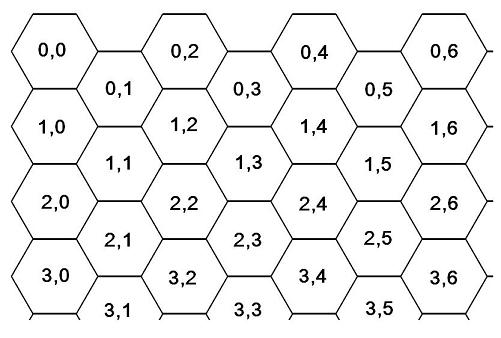
\includegraphics[width=10cm]{hex_array.jpg}

    \label{hexmatrix}

    \caption{Imagem mostrando o modo de enumeração dos terrenos}

\end{figure}


\section{Interfaces}

Aqui daremos uma breve explicação sobre as interfaces presentes no projeto:

\begin{itemize}

	\item \textbf{Programável}: Toda classe que implementa essa interface pode ser colocada dentro
	de um obejto do tipo \textbf{\color{red}Maquina}. Ou seja, quem implementa essa interface é
	todo aquele objeto que conterá uma máquina virtual. Por enquanto, só os robôs são programáveis,
	mas no futuro alguns terrenos poderão ser programáveis.

	\item \textbf{Empilhável}: Toda classe que implementa essa interface é tratada como um \emph{Empilhável},
	ou seja, objetos que a máquina virtual manipula em sua pilha de execução e em sua memória.

\end{itemize}

\section{Novas instruções}

Nessa fase, criamos novas instruções. Breve explicação sobre elas:

\begin{itemize}

	\item \textbf{ALO}: Aloca uma variável local, e empilha um objeto do tipo \textbf{\color{red}Endereço}.
	\item \textbf{GET}: Desempilha um \textbf{\color{red}Endereço}, e empilha o valor contido nesse Endereço.
	\item \textbf{SET}: Desempilha dois elementos da pilha. Se o segundo for do tipo \textbf{\color{red}Endereço},
	é colocado o valor do primeiro argumento desempilhado na variavel localizada no endereço desempilhado.
	\item \textbf{Chamadas ao sistema}: Atualmente, todas as chamadas ao sistema devem ser acompanhadas de um argumento indicando a direção. As direções podem ser: 1 - Cima, 2 - Direita superior, 3 - Direita inferior, 4 - Baixo, 5 - Esquerda inferior, 6 - Esquerda superior. As instruções implementadas são:
		\begin{itemize}

		\item[+] \textbf{WALK}: O robô tenta andar para a posição indicada
		\item[+] \textbf{COLLECT}: O robô tenta coletar cristais da posição indicada
		\item[+] \textbf{DROP}: O robô tenta deixar o cristal na posição desejada. Se a posição não for uma base, o cristal é retornado para seu ponto inicial.
		\item[+] \textbf{ATK}: O robô tenta atacar outro robo localizado na posição indicada.

		\end{itemize}

\end{itemize}


\section{Tradutor em Perl}

Para efeito de teste, adaptamos o montador em perl para gerar um arquivo Java que, ao ser executado, irá transformar os programas em linguagem de máquina para robôs e irá executar iterações da Arena até que não exista mais nenhum outro robô para ser executado.

Assim, para gerar esse arquivo em Java, chamado \textbf{\color{red}Main.java}, execute a seguinte linha de comando:
\begin{verbatim}

$>./montador.pl arquivo1 arquivo2 ... arquivoN

\end{verbatim}

\section{Modo de compilação}

Para compilar, execute o seguinte comando:

\begin{verbatim}

$> javac *.java

\end{verbatim}

Caso você tenha gerado o arquivo Main.java com o script em perl, para executar o programa, execute:

\begin{verbatim}

$> java Main

\end{verbatim}

\end{document}
